\documentclass{article}\usepackage[]{graphicx}\usepackage[]{color}
%% maxwidth is the original width if it is less than linewidth
%% otherwise use linewidth (to make sure the graphics do not exceed the margin)
\makeatletter
\def\maxwidth{ %
  \ifdim\Gin@nat@width>\linewidth
    \linewidth
  \else
    \Gin@nat@width
  \fi
}
\makeatother

\definecolor{fgcolor}{rgb}{0.345, 0.345, 0.345}
\newcommand{\hlnum}[1]{\textcolor[rgb]{0.686,0.059,0.569}{#1}}%
\newcommand{\hlstr}[1]{\textcolor[rgb]{0.192,0.494,0.8}{#1}}%
\newcommand{\hlcom}[1]{\textcolor[rgb]{0.678,0.584,0.686}{\textit{#1}}}%
\newcommand{\hlopt}[1]{\textcolor[rgb]{0,0,0}{#1}}%
\newcommand{\hlstd}[1]{\textcolor[rgb]{0.345,0.345,0.345}{#1}}%
\newcommand{\hlkwa}[1]{\textcolor[rgb]{0.161,0.373,0.58}{\textbf{#1}}}%
\newcommand{\hlkwb}[1]{\textcolor[rgb]{0.69,0.353,0.396}{#1}}%
\newcommand{\hlkwc}[1]{\textcolor[rgb]{0.333,0.667,0.333}{#1}}%
\newcommand{\hlkwd}[1]{\textcolor[rgb]{0.737,0.353,0.396}{\textbf{#1}}}%
\let\hlipl\hlkwb

\usepackage{framed}
\makeatletter
\newenvironment{kframe}{%
 \def\at@end@of@kframe{}%
 \ifinner\ifhmode%
  \def\at@end@of@kframe{\end{minipage}}%
  \begin{minipage}{\columnwidth}%
 \fi\fi%
 \def\FrameCommand##1{\hskip\@totalleftmargin \hskip-\fboxsep
 \colorbox{shadecolor}{##1}\hskip-\fboxsep
     % There is no \\@totalrightmargin, so:
     \hskip-\linewidth \hskip-\@totalleftmargin \hskip\columnwidth}%
 \MakeFramed {\advance\hsize-\width
   \@totalleftmargin\z@ \linewidth\hsize
   \@setminipage}}%
 {\par\unskip\endMakeFramed%
 \at@end@of@kframe}
\makeatother

\definecolor{shadecolor}{rgb}{.97, .97, .97}
\definecolor{messagecolor}{rgb}{0, 0, 0}
\definecolor{warningcolor}{rgb}{1, 0, 1}
\definecolor{errorcolor}{rgb}{1, 0, 0}
\newenvironment{knitrout}{}{} % an empty environment to be redefined in TeX

\usepackage{alltt}
\usepackage[utf8]{inputenc}
\usepackage{hyperref}
\hypersetup{
  linktocpage,
  colorlinks=true, 
  linkcolor=blue,
  citecolor=blue,
  filecolor=blue,
  urlcolor=blue
}
\IfFileExists{upquote.sty}{\usepackage{upquote}}{}
\begin{document}

\title{Acetilation}
\author{Lucas Michel Todó}
\maketitle
\tableofcontents
\clearpage







@
\begin{knitrout}
\definecolor{shadecolor}{rgb}{0.969, 0.969, 0.969}\color{fgcolor}
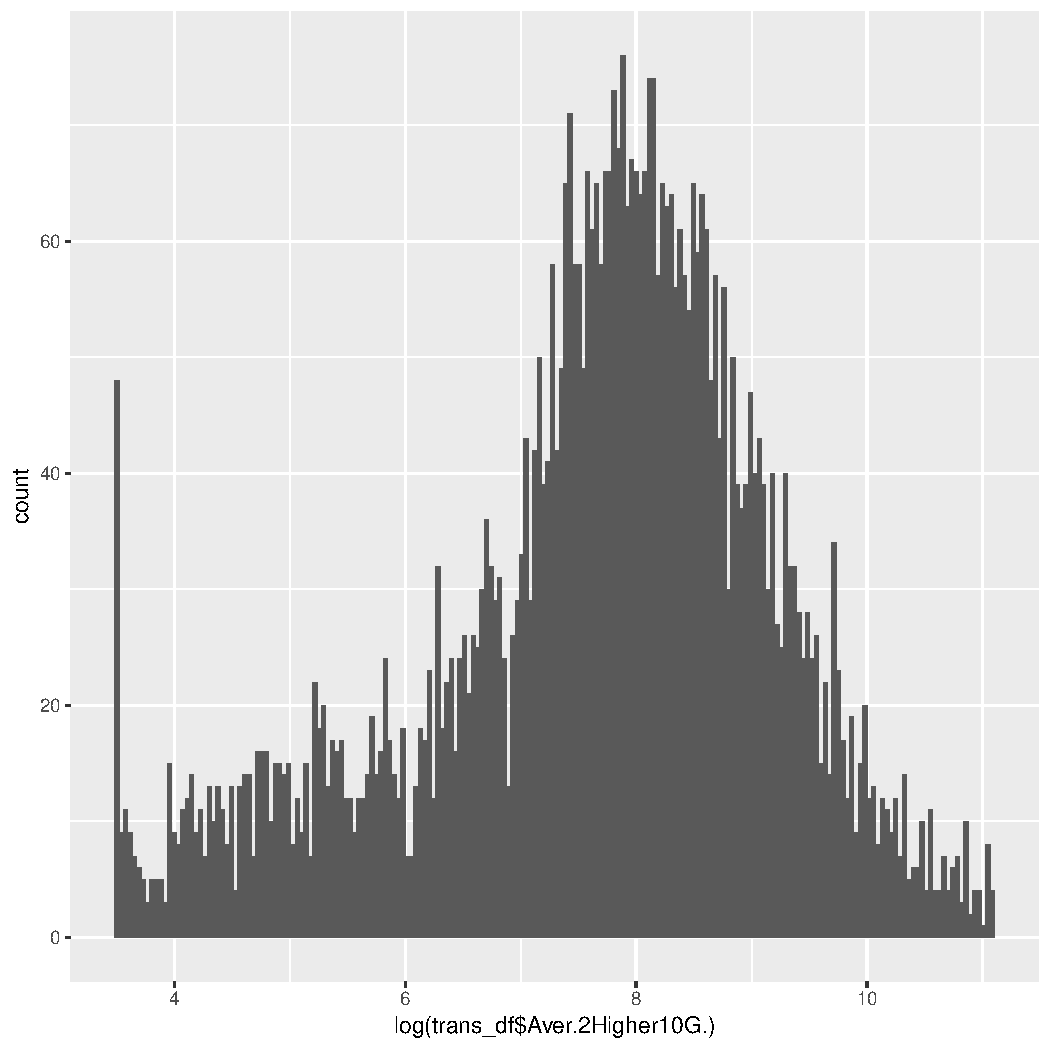
\includegraphics[width=\maxwidth]{figure/import_status_data-1} 

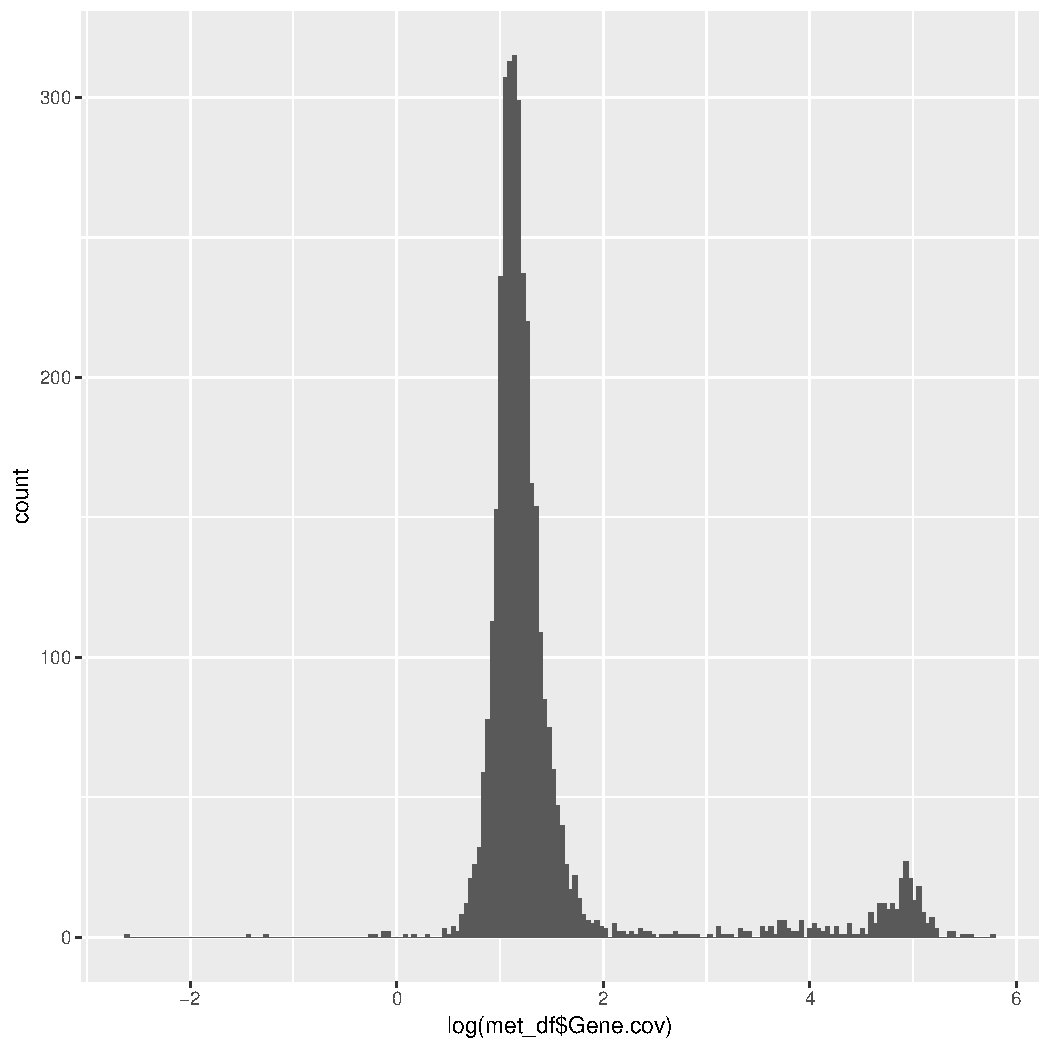
\includegraphics[width=\maxwidth]{figure/import_status_data-2} 
\begin{kframe}\begin{verbatim}
## 
## FALSE  TRUE 
##   214    74
## 
## FALSE  TRUE 
##    61    74
\end{verbatim}
\end{kframe}
\end{knitrout}

\section{Histograms}
\subsection{log(Ac) All}
\begin{knitrout}
\definecolor{shadecolor}{rgb}{0.969, 0.969, 0.969}\color{fgcolor}
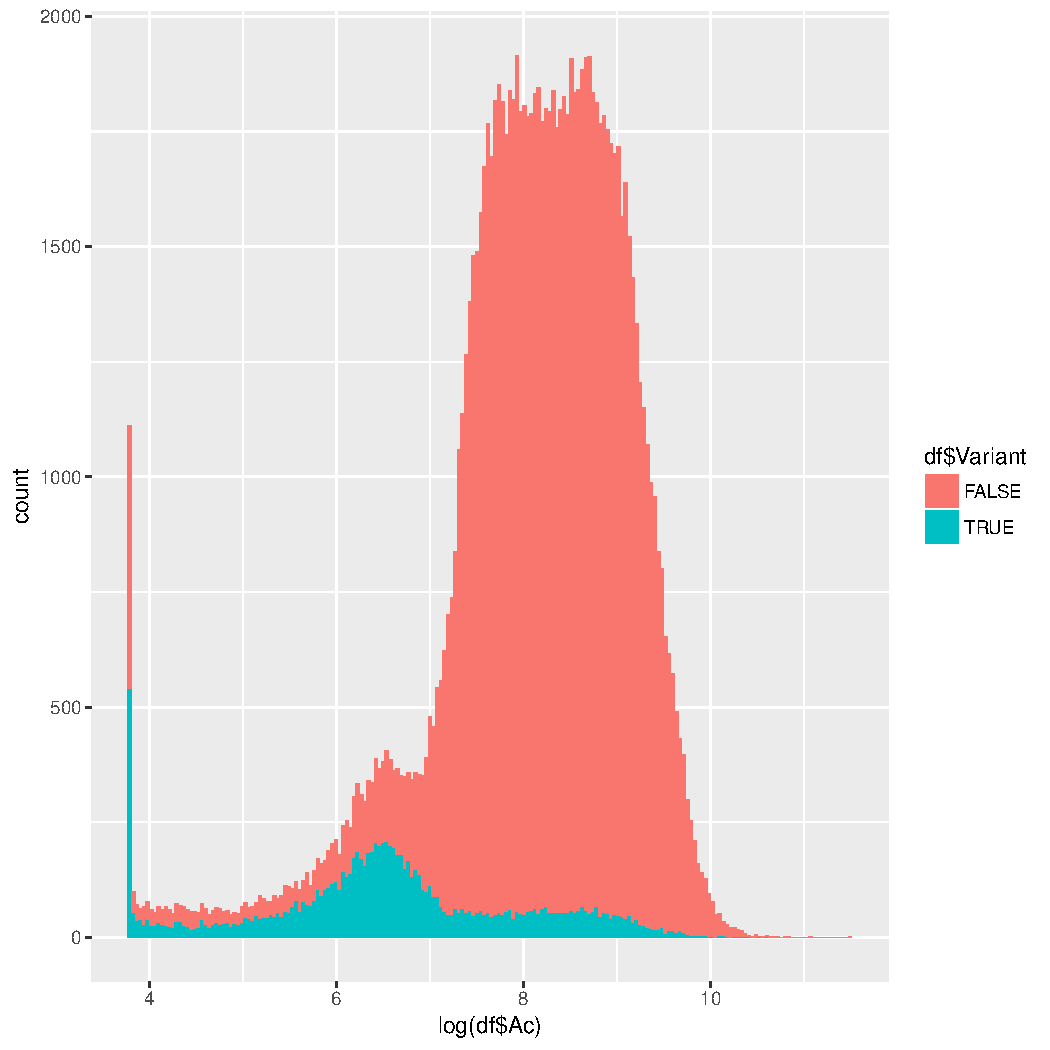
\includegraphics[width=1\linewidth]{figure/dens_all-1} 

\end{knitrout}
\clearpage
\subsection{log(Ac) 5'}
\begin{knitrout}
\definecolor{shadecolor}{rgb}{0.969, 0.969, 0.969}\color{fgcolor}
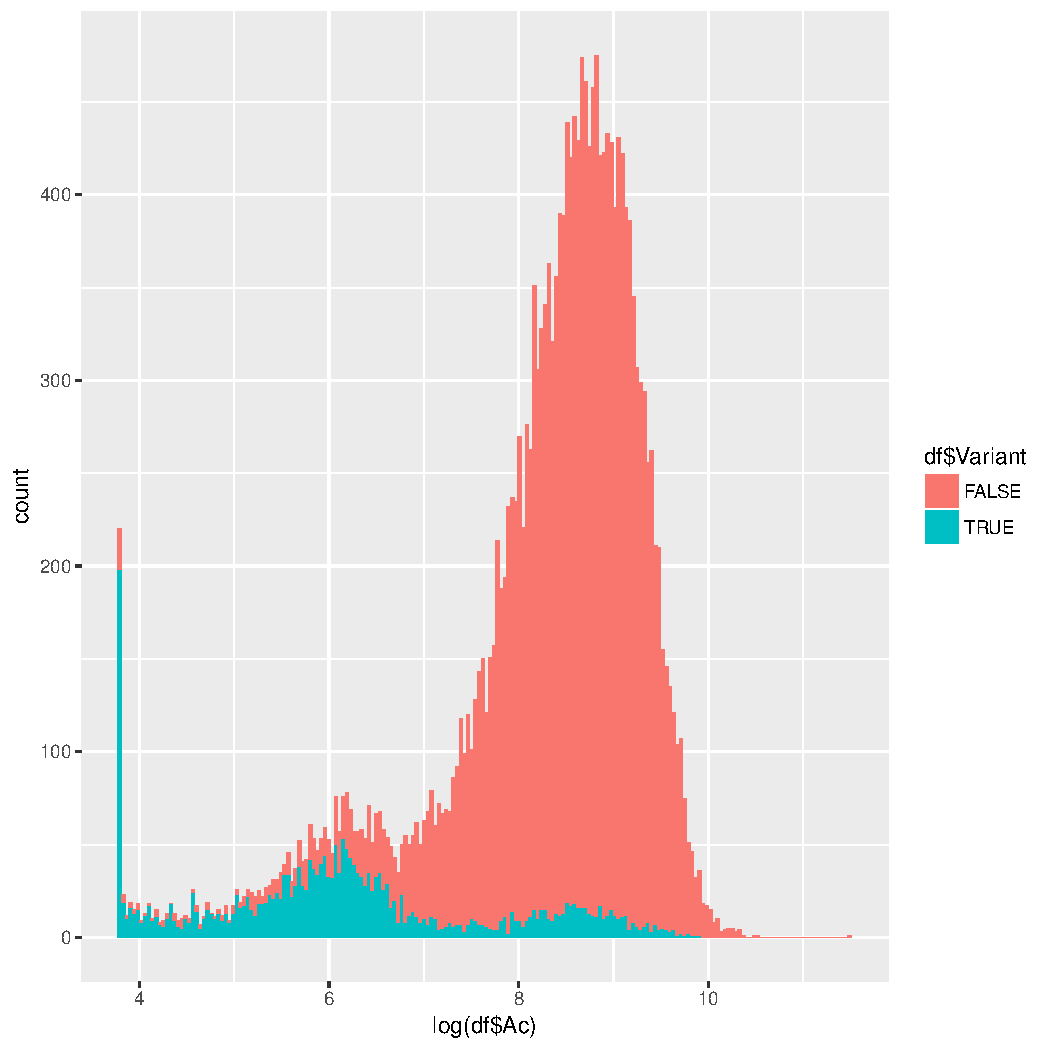
\includegraphics[width=1\linewidth]{figure/dens_5-1} 

\end{knitrout}
\clearpage
\subsection{log(Ac) 3'}
\begin{knitrout}
\definecolor{shadecolor}{rgb}{0.969, 0.969, 0.969}\color{fgcolor}
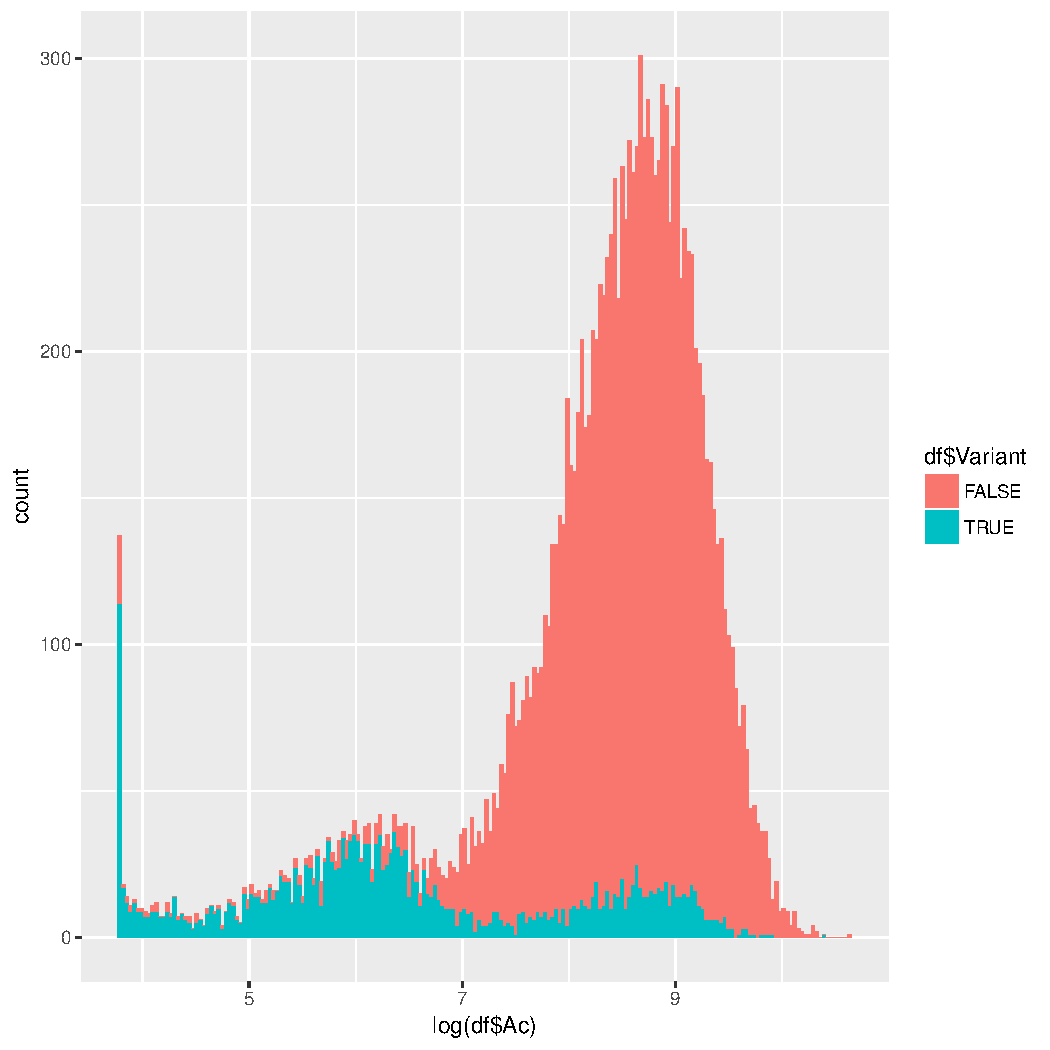
\includegraphics[width=1\linewidth]{figure/dens_3-1} 

\end{knitrout}
\clearpage
\subsection{log(Ac) ORF}
\begin{knitrout}
\definecolor{shadecolor}{rgb}{0.969, 0.969, 0.969}\color{fgcolor}
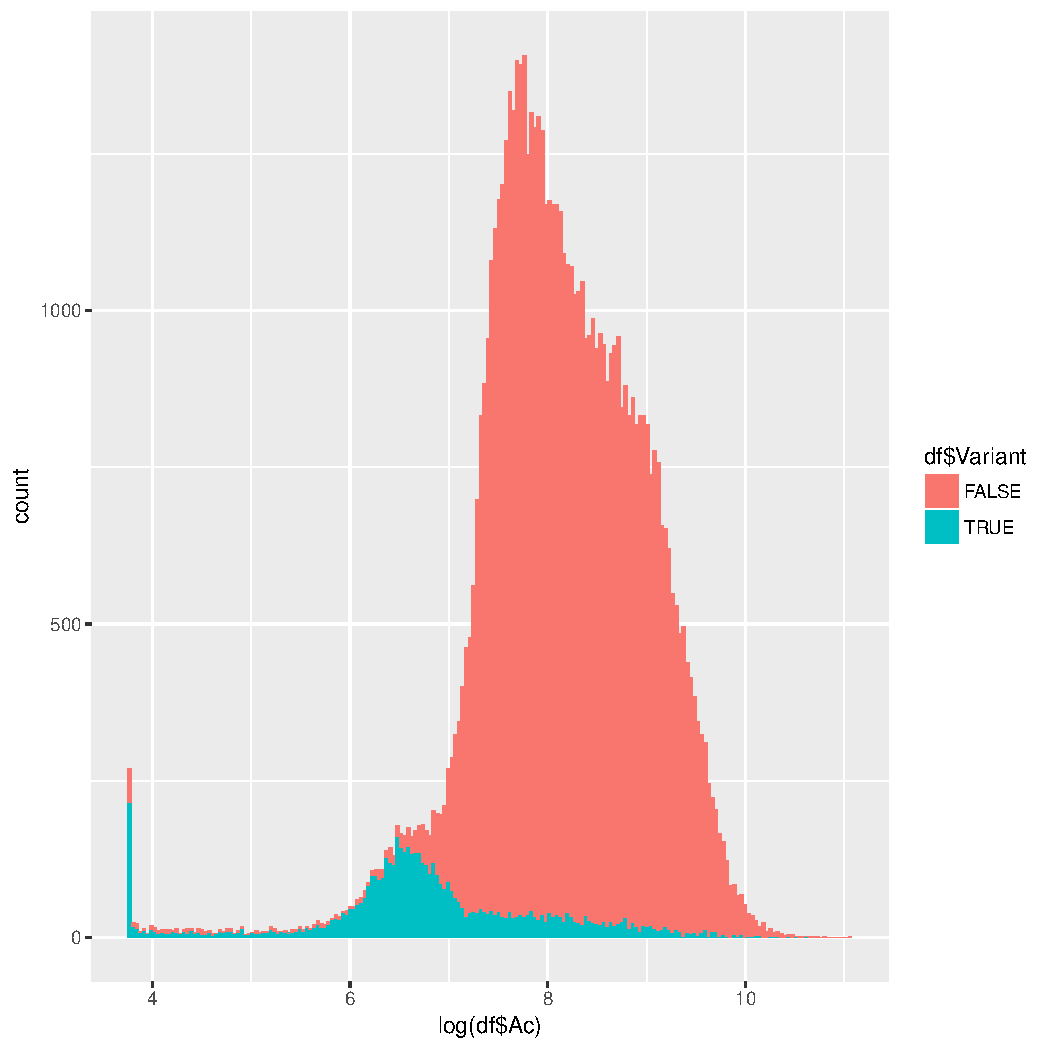
\includegraphics[width=1\linewidth]{figure/dens_ORF-1} 

\end{knitrout}
\clearpage
\subsection{log(Met) All}
\begin{knitrout}
\definecolor{shadecolor}{rgb}{0.969, 0.969, 0.969}\color{fgcolor}
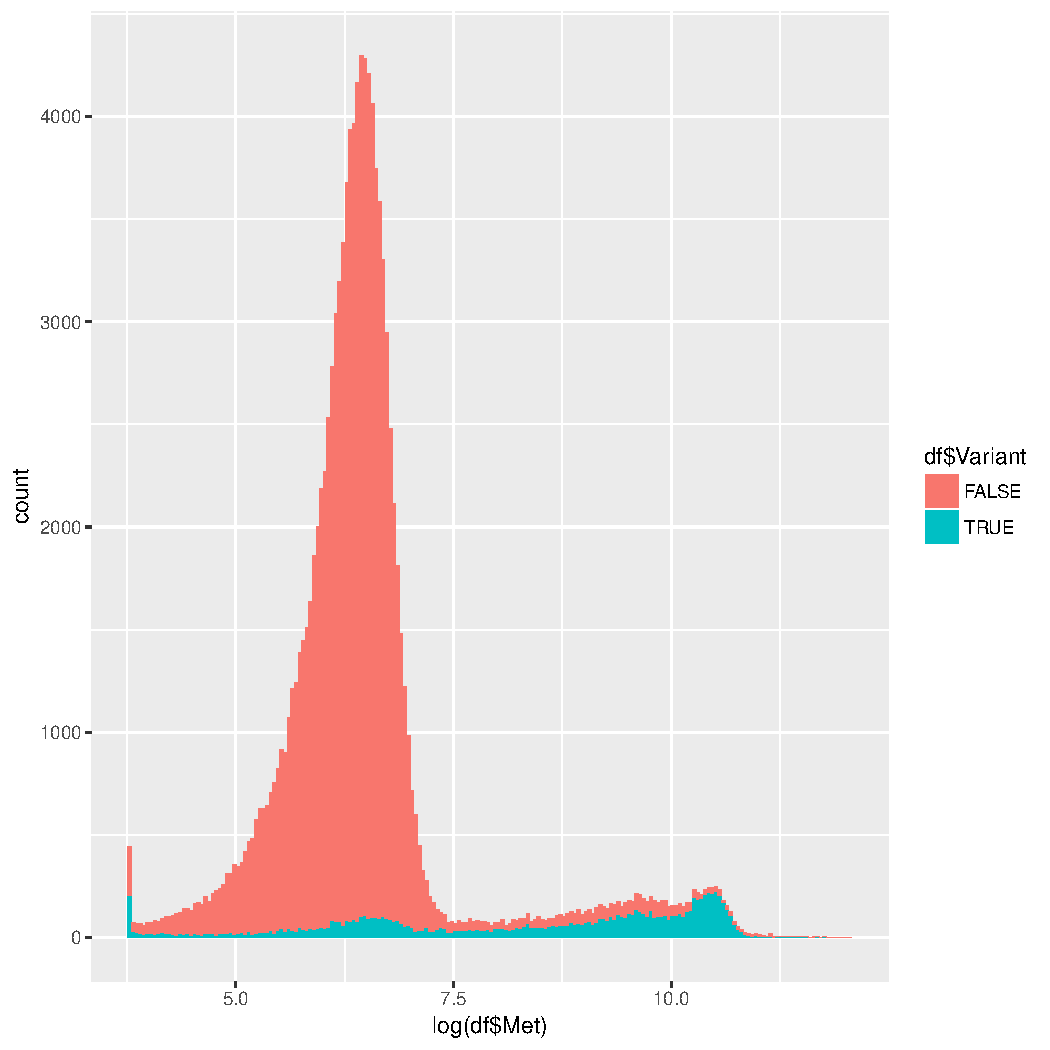
\includegraphics[width=1\linewidth]{figure/dens_all_met-1} 

\end{knitrout}
\clearpage
\subsection{log(Met) 5'}
\begin{knitrout}
\definecolor{shadecolor}{rgb}{0.969, 0.969, 0.969}\color{fgcolor}
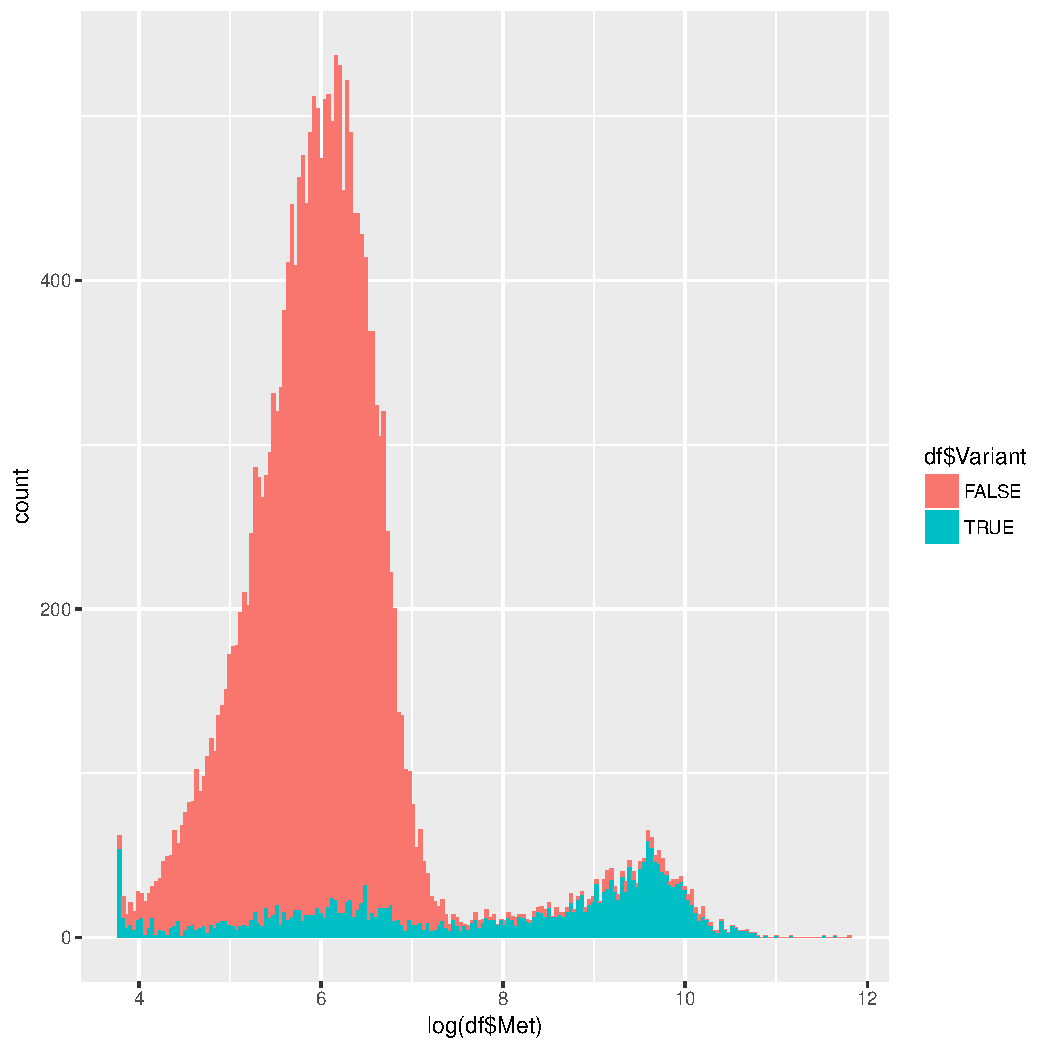
\includegraphics[width=1\linewidth]{figure/dens_5_met-1} 

\end{knitrout}
\clearpage
\subsection{log(Met) ORF}
\begin{knitrout}
\definecolor{shadecolor}{rgb}{0.969, 0.969, 0.969}\color{fgcolor}
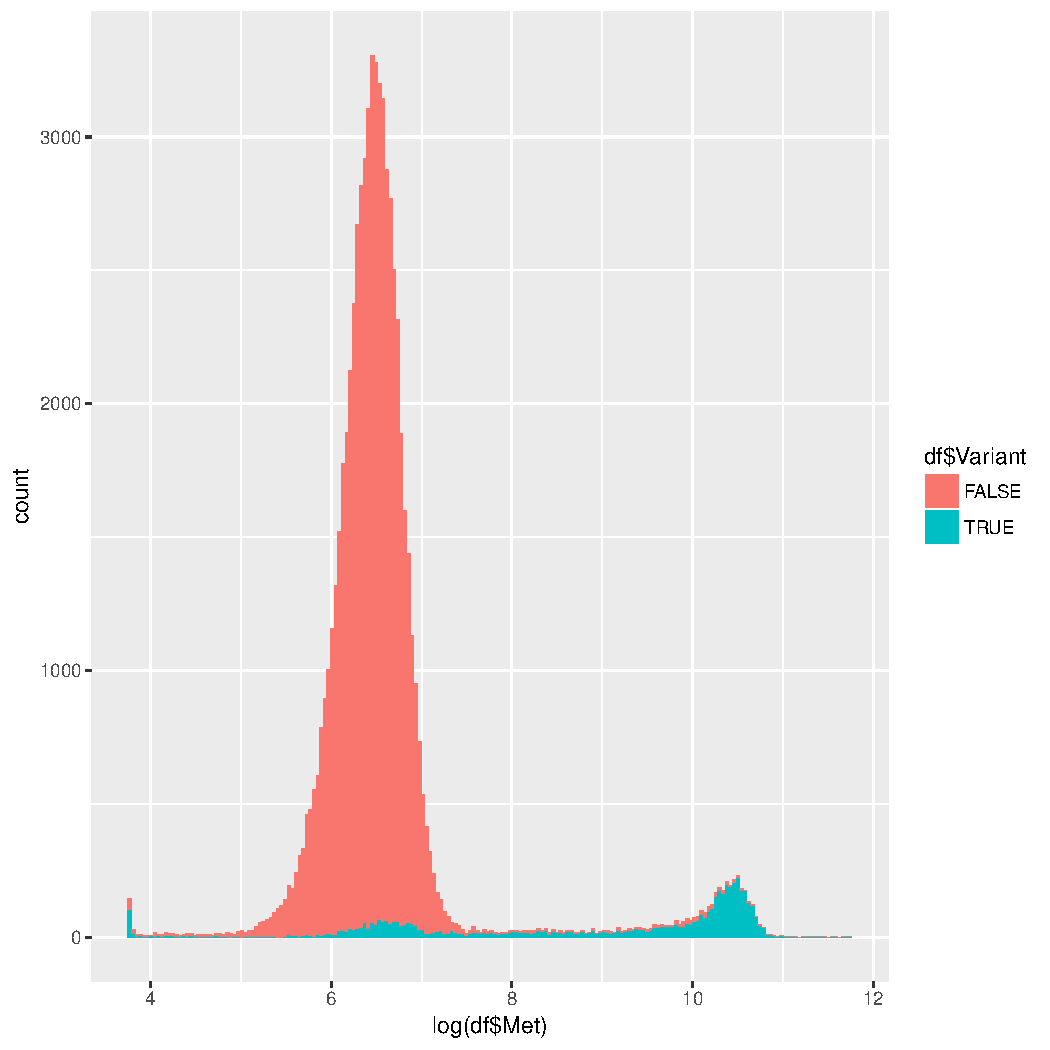
\includegraphics[width=1\linewidth]{figure/dens_ORF_met-1} 

\end{knitrout}
\clearpage
\subsection{log(Ac) 3'}
\begin{knitrout}
\definecolor{shadecolor}{rgb}{0.969, 0.969, 0.969}\color{fgcolor}
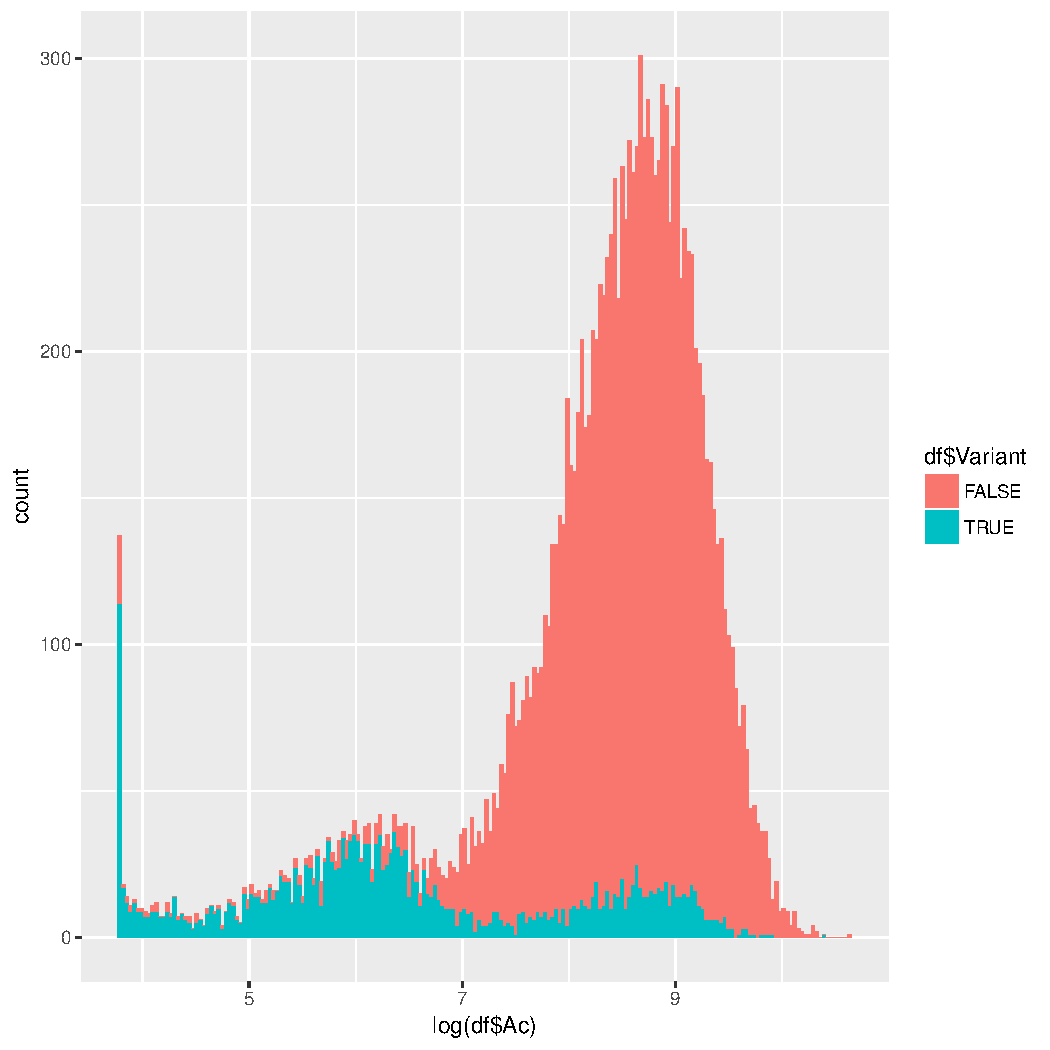
\includegraphics[width=1\linewidth]{figure/dens_3_met-1} 

\end{knitrout}

\section{Metilation/Acetilation plots}

Genes have been classified as variant or not on the basis of a previous study.

Fragments have been set to "noexprs" if transcription value is under threshold (<4).
Fragments have been set to "silenced" if methilation value is over threshold(>3).
\begin{knitrout}
\definecolor{shadecolor}{rgb}{0.969, 0.969, 0.969}\color{fgcolor}\begin{kframe}
\begin{verbatim}
## 
##  FALSE   TRUE 
## 114212   2445
\end{verbatim}
\end{kframe}
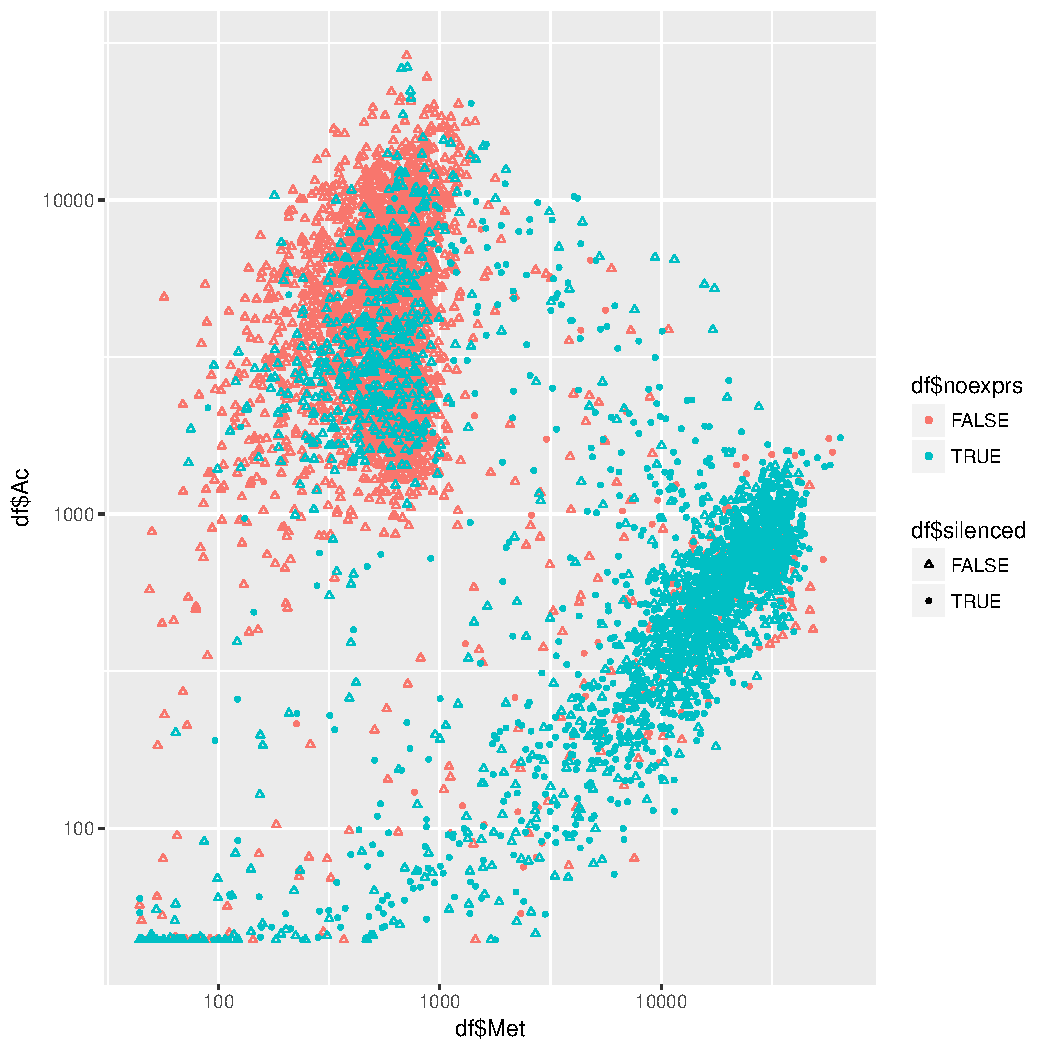
\includegraphics[width=1\linewidth]{figure/ac_met_log-1} 

\end{knitrout}
\clearpage
Here we have highlited those genes that are "variant" (as shown in previous studies) and differentially expressed between 10G and 1.2B. Variant genes which are overexpressed have been set to "variant active" and viceversa.

10G and 1.2B fragments have been pooled toghether for the grafic. Blurred point correspond to fragments representing the rest of genes (those that are not diferentially expressed). 
\begin{knitrout}
\definecolor{shadecolor}{rgb}{0.969, 0.969, 0.969}\color{fgcolor}
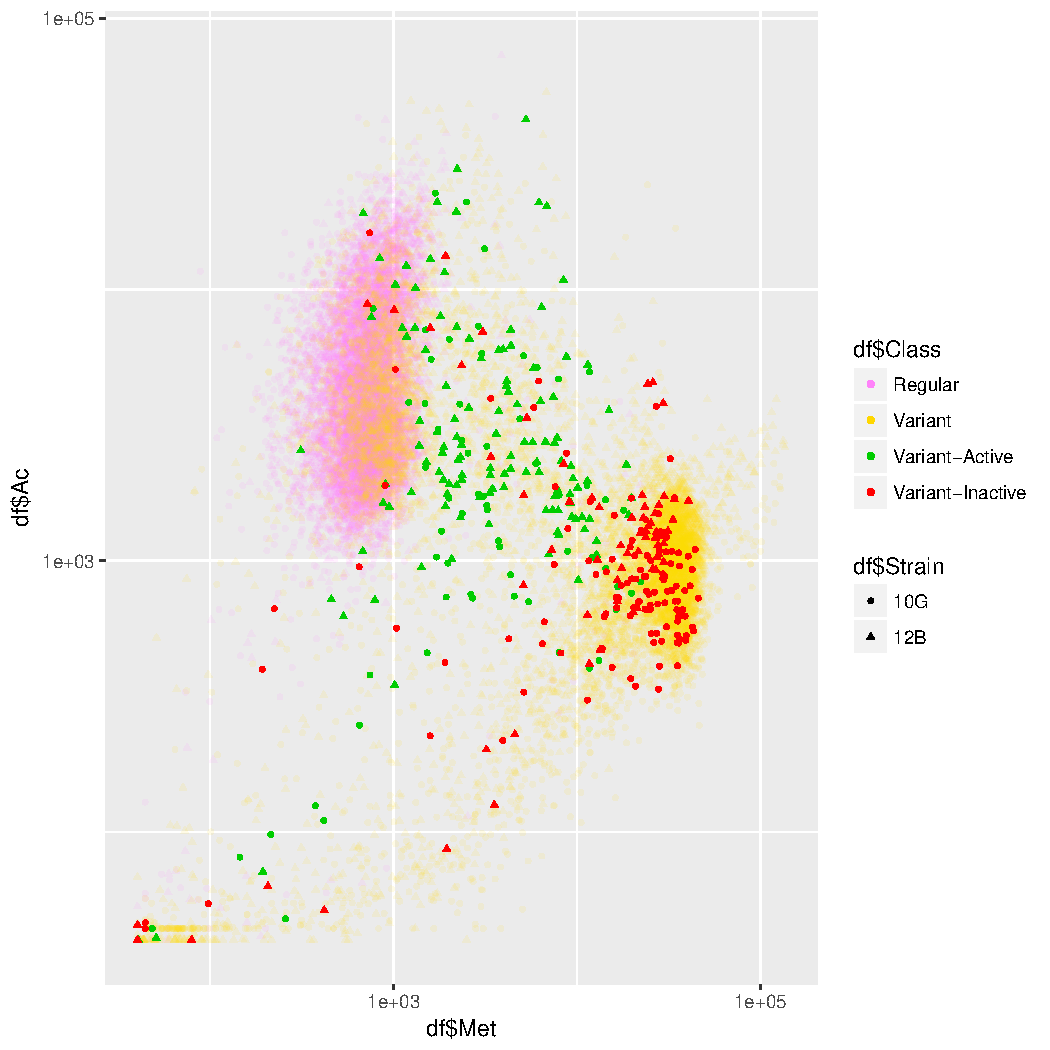
\includegraphics[width=1\linewidth]{figure/ac_met_log_status_10G_12B-1} 

\end{knitrout}
\begin{knitrout}
\definecolor{shadecolor}{rgb}{0.969, 0.969, 0.969}\color{fgcolor}\begin{kframe}
\begin{verbatim}
## 
##  FALSE   TRUE 
## 105873  10784
## Analysis of Deviance Table
## 
## Model 1: Variant ~ Ac + Met + Type + Start + Stop + silenced + noexprs
## Model 2: Variant ~ Ac + Met + Type + Start + Stop
##   Resid. Df Resid. Dev Df Deviance  Pr(>Chi)    
## 1      8477     5498.4                          
## 2      8479     6141.6 -2  -643.16 < 2.2e-16 ***
## ---
## Signif. codes:  0 '***' 0.001 '**' 0.01 '*' 0.05 '.' 0.1 ' ' 1
## 
## Call:
## glm(formula = Variant ~ Ac + Met + Type + Start + Stop + silenced + 
##     noexprs, family = binomial(link = "logit"), data = train_df)
## 
## Deviance Residuals: 
##     Min       1Q   Median       3Q      Max  
## -5.6138  -0.7408   0.0020   0.1488   2.7447  
## 
## Coefficients: (1 not defined because of singularities)
##                Estimate Std. Error z value Pr(>|z|)    
## (Intercept)   6.643e-01  1.012e-01   6.566 5.17e-11 ***
## Ac           -1.340e-04  9.630e-06 -13.916  < 2e-16 ***
## Met           3.826e-04  3.141e-05  12.180  < 2e-16 ***
## Type5prima   -2.894e-01  1.016e-01  -2.847  0.00441 ** 
## TypeORF      -1.050e+00  8.838e-02 -11.880  < 2e-16 ***
## Typeother    -2.885e+01  2.288e+02  -0.126  0.89963    
## Start        -2.339e-07  4.308e-08  -5.430 5.62e-08 ***
## Stop                 NA         NA      NA       NA    
## silencedTRUE  4.138e+00  3.254e-01  12.715  < 2e-16 ***
## noexprsTRUE   1.642e+00  2.608e-01   6.296 3.05e-10 ***
## ---
## Signif. codes:  0 '***' 0.001 '**' 0.01 '*' 0.05 '.' 0.1 ' ' 1
## 
## (Dispersion parameter for binomial family taken to be 1)
## 
##     Null deviance: 11193.5  on 8485  degrees of freedom
## Residual deviance:  5498.4  on 8477  degrees of freedom
## AIC: 5516.4
## 
## Number of Fisher Scoring iterations: 17
##        
##         FALSE TRUE
##   FALSE  2964  252
##   TRUE   1060 4387
## [1] "Accuracy 0.848551310169687"
\end{verbatim}


{\ttfamily\noindent\bfseries\color{errorcolor}{\#\# Error in `[<-.data.frame`(`*tmp*`, "{}all\_0.5"{}, value = c(0, 1, 1, 0, 0, : replacement has 8845 rows, data has 8663}}\begin{verbatim}
## [1] "Accuracy of null model NaN"
\end{verbatim}


{\ttfamily\noindent\itshape\color{messagecolor}{\#\# Loading required package: gplots}}

{\ttfamily\noindent\itshape\color{messagecolor}{\#\# \\\#\# Attaching package: 'gplots'}}

{\ttfamily\noindent\itshape\color{messagecolor}{\#\# The following object is masked from 'package:stats':\\\#\# \\\#\#\ \ \ \  lowess}}\end{kframe}
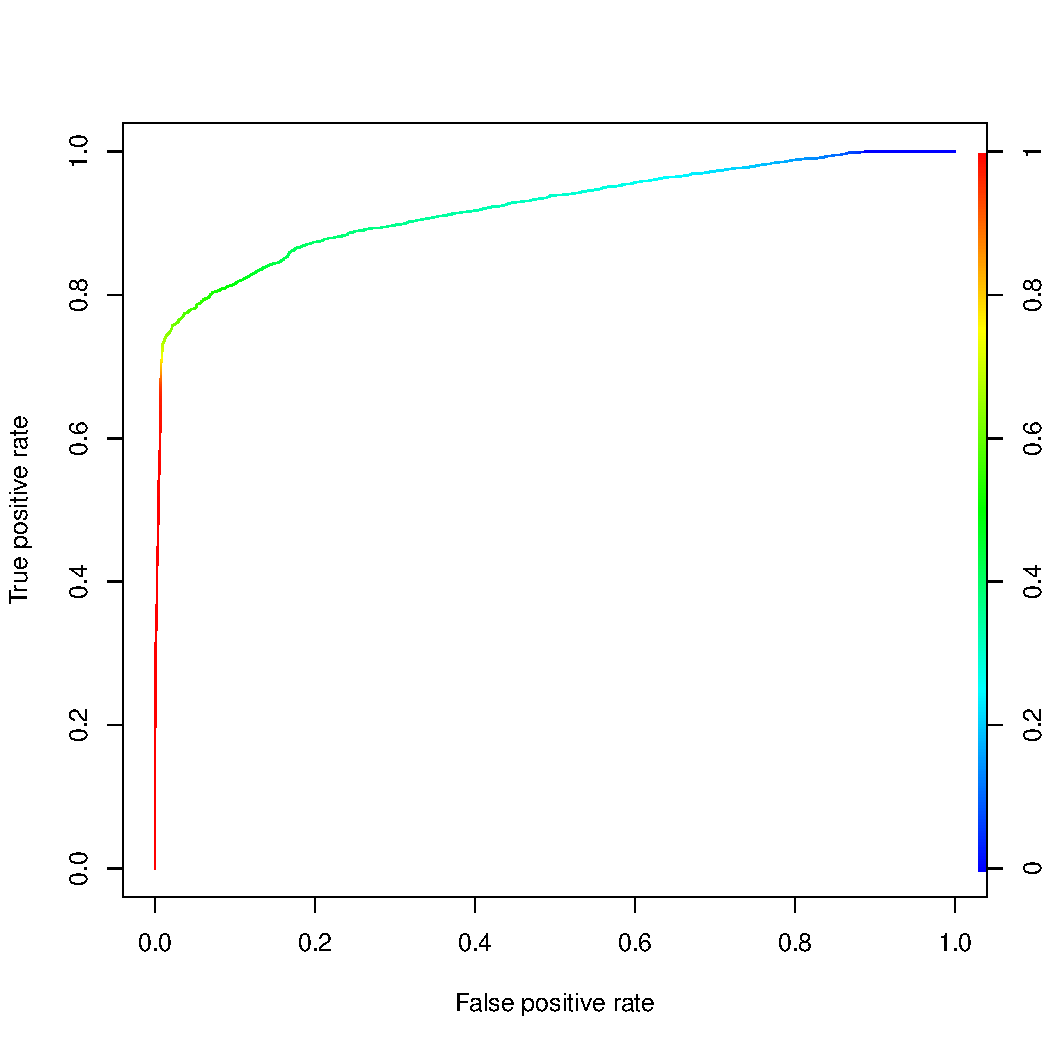
\includegraphics[width=\maxwidth]{figure/model-1} 
\begin{kframe}\begin{verbatim}
## 
## 3prima 5prima    ORF  other 
##    140     89     21      2
## 
## 3prima 5prima    ORF 
##    171    213    676
##           llh       llhNull            G2      McFadden          r2ML 
## -2749.2229441 -5596.7623637  5695.0788391     0.5087833     0.4888615 
##          r2CU 
##     0.6672848
\end{verbatim}
\end{kframe}
\end{knitrout}



\end{document}
